\subsection{The \HTSR Setup}
\label{sxn:htsr_setup}

We can write the \EnergyLandscape function 
(or NN output function) for a 
%%\emph{\Typical} 
NN with $L$ layers as
\begin{equation}
\label{eqn:dnn_energy}
\NNOUT:=h_{L}(\mathbf{W}_{L}\times h_{L-1}(\mathbf{W}_{L-1}\times(\cdots)+\mathbf{b}_{L-1})+\mathbf{b}_{L}) 
\end{equation}
with activation functions $h_{l}(\cdot)$, and with weight matrices and biases $\mathbf{W}_{l}$ and $\mathbf{b}_{l}$.%
\footnote{The Energy Landscape function $\NNOUT$ acts on a data instance and generates a list of energies, or un-normalized probabilities;
~\cite{MM18_TR_JMLRversion}.
This notation was chosen to make an analogy with Random Energy Models (REM)
from spin-glass and protein folding theories~\cite{DerridaREM1981, BryngelsonWolynesPNAS1987}.
}
For simplicity of exposition here (\HTSR can be applied much more broadly), we ignore the structural details of the layers (dense or not, convolutions or not, residual/skip connections, etc.).
We also ignore the biases $b_{l}$ (because they can be subsumed into the weight matrices),
and we treat each layer as though it contains a single weight matrix $\mathbf{W}_{L}$.
We imagine training (or fine-tuning) this model on labeled data $\{\mathbf{x}_{\mu},y_{\mu}\}\in\mathcal{D}$, where $ \mathbf{x}_\mu $ is the $\mu$-th input vector and $y_\mu$ is its corresponding label (e.g., for binary classification, $y_{\mu}\in\{-1,1\}$).
We expect to use backprop via some variant of stochastic gradient descent (SGD) to minimize some loss functional, $\mathcal{L}$ (such as $\ell_2$, cross-entropy, etc.):  
\begin{equation}
\underset{\mathbf{W}_{l},\mathbf{b}_{l}}{\argmin}\;\sum_{\mu}\mathcal{L}[\NNOUT(\mathbf{x}_{\mu}),y_{\mu}]+\Omega ,
\label{eqn:dnn_opt}
\end{equation}
where, $\Omega$ denotes some explicit regularizer (such as an $\ell_1$ or $\ell_2$ constraint on layer weight matrices) or some implicit regularization procedure (such as clipping the weight matrices or applying dropout).

Given a real-valued $N\times M$ layer weight matrix $\mathbf{W}$ (dropping the subscript), let $\mathbf{X}$ be the $M \times M$ layer \emph{\CorrelationMatrix}:
\begin{equation}
\mathbf{X}:=\dfrac{1}{N}\mathbf{W}^{\top}\mathbf{W} .
\label{eqn:X}
\end{equation}

\noindent
The \EmpiricalSpectralDensity (ESD) of $\mathbf{W}$, denoted $\rho^{emp}(\lambda)$, is formed from the M eigenvalues $\lambda_{j}$ of $\mathbf{X}$:
\begin{equation}
\rho_{emp}(\lambda):=\sum_{j=1}^{M}\delta(\lambda-\lambda_{j}) .
\label{eqn:rho}
\end{equation}
Given a model, we can compute the ESDs of all of its layers, as well as other metrics below,
with the open-source \WW tool~\cite{WW}.%
\footnote{For practical purposes, the \WW tool computes $\rho^{emp}(\lambda)$ by forming the Singular Value Decomposition (SVD) of the layer weight matrices $\mathbf{W}$, computing the eigenvalues $\lambda=\sigma^{2}$ from the singular values $\sigma$, and (when useful) smoothing them with a Kernel Density Estimator (KDE). For some calculations, such as the \TRACELOG condition, we must also select the appropriate normalization of $\mathbf{W}$.}


Based on empirical results based on thousands of pretrained models and tens of thousands of layers~\cite{MM18_TR_JMLRversion,MM20a_trends_NatComm,MM21a_simpsons_TR,YTHx23_KDD}, 
it is generally observed that the 
best performing NNs have ESDs that are HT, and the \emph{tails} of these ESDs, $\rho_{tail}(\lambda)$, can be well fit to a PL, beyond some cutoff $\lambda\ge\LambdaMin$.%
\footnote{Doing a large meta-analysis like this is tricky; but see~\cite{MM18_TR_JMLRversion,MM20a_trends_NatComm,MM21a_simpsons_TR,YTHx23_KDD}.  The \WW~tool provides a systematic, reproducible way to compute a PL fit (using an MLE method of Clauset et al.~\cite{CSN09_powerlaw}), as well other model metrics, including the \SPECTRALNORM, \RANDDIST, and \ALPHAHAT metrics~\cite{MM20a_trends_NatComm}.  Also, the ESD $\rho(\lambda)_{tail}$ is sometimes better fit by a Truncated \PowerLaw (TPL), due to finite-size effects.
(again, this is important in practice, but we ignore this complexity in this initial discussion of \SETOL. ) }
For a PL fit,
\begin{equation}
\rho_{tail}(\lambda):=\rho^{emp}(\lambda\ge\LambdaMin)\sim\lambda^{-\alpha} ,
\label{eqn:rho_tail}
\end{equation}
where $\LambdaMin$ is where the tail of the ESD starts (i.e., it is not the minimum eigenvalue, but the minimum eigenvalue in the tail of the ESD). 
See Figure~\ref{fig:log-esds}.
As such, the tail of the ESD ``starts'' at some value $\LambdaMin$, called $xmin$ here, and it continues until the 
maximum eigenvalue $\LambdaMax$, called $xmax$ here
(labeled $xmax$ in the figure, shown by the orange line).
We estimate $xmin$ and $\alpha$ jointly, using the method of~\cite{CSN09_powerlaw}, 
as implemented in the \texttt{powerlaw} python package~\cite{ABP14}, 
which is also integrated into the open-source \WW tool~\cite{MM20a_trends_NatComm, WW}.%
\footnote{The authors of~\cite{Thamm2022} failed to find evidence of a PL-like distribution in NN weight matrices, which is 
likely to be the case when $\alpha$ and $xmin$ are not estimated \emph{jointly}, as can be seen in Figure~\ref{fig:xmin-DKS-esd}.  }


%%While the ESD can be computed as a histogram of eigenvalues, it is often more convenient to represent it using a kernel density estimator (KDE).


\begin{figure}[t] %[h]
    \centering
    \subfigure[Log-Log ESD]{
      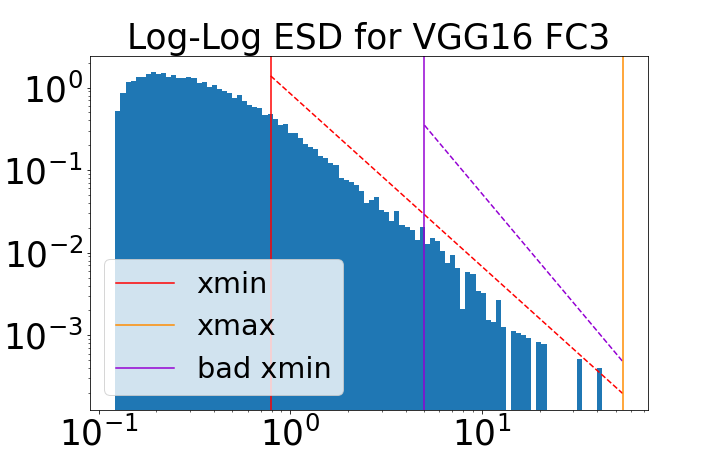
\includegraphics[width=7cm]{./img/fig1-1a.png}
      \label{fig:log-log-esd}
    }
    \subfigure[Lin-Lin ESD]{
      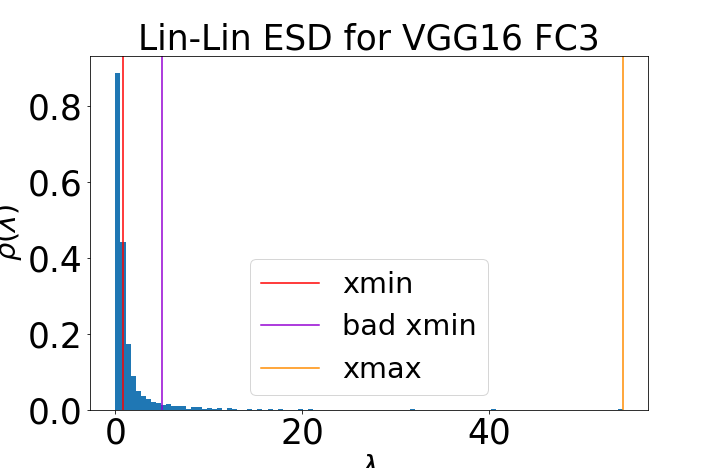
\includegraphics[width=7cm]{./img/fig1-1b.png}
      \label{fig:lin-lin-esd}
    }
    \subfigure[Log-Lin ESD]{
      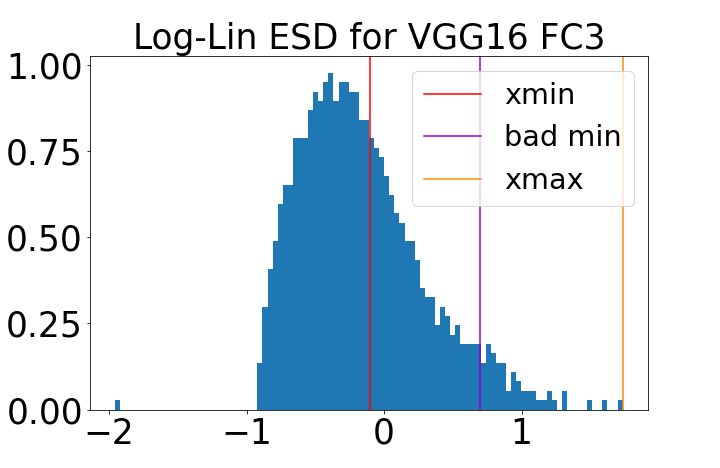
\includegraphics[width=7cm]{./img/fig1-1c.png}
      \label{fig:log-lin-esd}
    }
    \subfigure[$\LambdaMin$ vs KS distance]{
      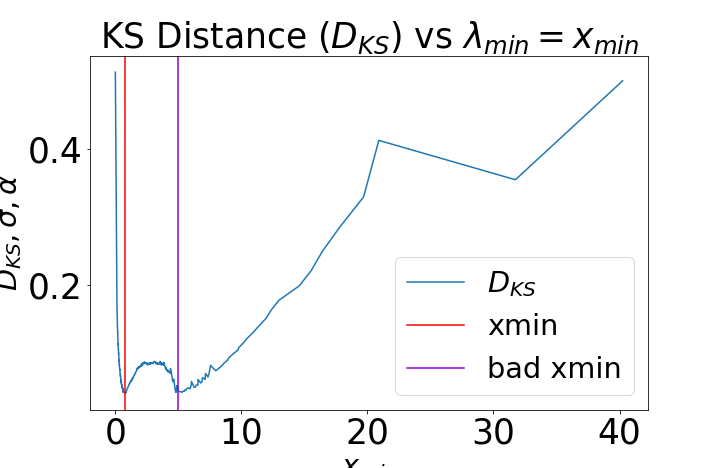
\includegraphics[width=7cm]{./img/fig1-1d.png}
      \label{fig:xmin-DKS-esd}
    }                                     
    \caption{\textbf{Fitting ESDs within \HTSR.} 
         Depiction of the ESD and results of PL fits for a typical well-trained layer of a modern NN (FC3 of VGG19), including both the actual and good PL fit (red) and a hypothetical bad PL fit (purple). 
         The same ESD is plotted on a Log-Log (a), Lin-Lin (b) and Log-Lin (c) scales.
         (d) depicts how the start of the PL tail, $\LambdaMin$, varies with the quality of the PL fit (the $D_{KS}$ distance). 
         All plots are generated using the open-source \WW tool. 
         See the main text for details.
    }
  \label{fig:log-esds}
\end{figure}   


%% %Figure~\ref{fig:log-esds} (from Figure~1 of~\cite{MM21a_simpsons_TR}) displays layer ESD plots for a \Typical layer $\mathbf{W}$,
%% %on different scales (\ref{fig:log-log-esd}, \ref{fig:lin-lin-esd}, \ref{fig:log-lin-esd}),
%% %along with the quality of fit ($D_{KS}$ vs. $x_min$, \ref{fig:xmin-DKS-esd}), as generated with the~\WW~tool,
%% %\footnote{The \WW~tool finds the best PL fit automatically and reproducibly.}

\paragraph{Fitting ESDs.}
Choosing the start of the tail, $\LambdaMin$, is important for \HTSR (and it will be very important for \SETOL, as we will describe below).
See Figure~\ref{fig:log-esds} for a depiction of how this was done within \HTSR theory.
Figures~\ref{fig:log-log-esd}-\ref{fig:log-lin-esd} show the results of both a ``good fit'' and a ``bad fit'' on the same ESD,
while Figure~\ref{fig:xmin-DKS-esd} indicates the quality of fit.
For the good fit, the start of the tail is the optimal value $\LambdaMin=xmin$ (in red); and for the bad fit, it is a suboptimal $bad\;xmin$ (purple).
Figure~\ref{fig:xmin-DKS-esd} depicts how the best fit is determined; it plots $xmin=\LambdaMin$ versus the $D_{KS}$ 
value, which is the Kolmogorov-Smirnov (KS) distance between the PL fit and the empirical data~\cite{CSN09_powerlaw}.
Notice that there are two nearly degenerate minima on Figure~\ref{fig:xmin-DKS-esd}, corresponding to the good fit and the bad fit. 
It is not uncommon to face such practical challenges, as real-world ESDs are often slightly deformed from a perfect PL density, e.g.,
they may have two or more near degenerate solutions on the KS plots (d).
(They may also have anomalously large eigenvalues; this is discussed in more detail in Section~\ref{sxn:HT_ESDs}.)

%%Additionally, some PL fits may require ignoring anamalously large eigenvalues, called ``\DragonKings'' in certain communities~\cite{sornette2009dragonkings}.
%%the \WW~tool can do this automatically.

When one finds a good PL fit for the ESD of a layer $\mathbf{W}$,
it provides information about the \SHAPE~and \SCALE~of the ESD of that layer.
In particular: 
the \SPECTRALNORM, $\lambda_{max}$, being a matrix norm, is a measure of the size \SCALE~of the ESD~\cite{MM21a_simpsons_TR}; 
the fitted PL exponent \ALPHA, $\alpha$, being the slope of the tail of the ESD on a Log-Log plot, describes the \SHAPE~of the ESD; and
the \WW \ALPHAHAT~metric combines \SHAPE~and \SCALE~information.
Also, as opposed to other applications of PL fits~\cite{CSN09_powerlaw,BouchaudPotters03}, in our analysis,
the start of the tail, $\LambdaMin=\LambdaPLmin$, plays a particularly important role because it
identifies the subspace of the strongest generalizing eigencomponents (i.e., $\XECS$, below) in each layer.

\begin{table}[t] %[ht!]
\begin{center}
  \begin{tabular}{| l | c | c | r | }
    \hline
    HT/\RMT Universality class & $\mu$ range   & $\alpha$ range    & Best Fit  \\ \hline \hline
    RandomLike            & NA            & NA                & MP        \\ \hline
    Bulk+Spikes           & NA            & NA                & MP+Spikes \\ \hline
    Weakly Heavy Tailed   & $\mu > 4$     & $\alpha>6$        & PL        \\ \hline
    Heavy (Fat) Tailed    & $\mu\in(2,4)$ & $\alpha\in(2,6)$  & PL        \\ \hline
    Very Heavy Tailed     & $\mu\in(0,2)$ & $\alpha\in(1,2) $ & (T)PL     \\ \hline
    Rank Collapse       & NA            & NA                & NA        \\ \hline
  \end{tabular}
\end{center}
\caption{\HTSR~Heavy-Tailed Universality classes of \RMT. See Table~1 of \cite{MM18_TR_JMLRversion} for more details.    }
\label{tab:Uclass}
\end{table}

